
\section{Невронски мрежи}

Имплементација на алгоритмот за повратна пропагација за учење на параметрите на
невронската мрежа. Овој алгоритам ќе го искористиме за препознавање на ракописно
напишани цифри. Ова е корисно во автоматско читање на поштенски кодови, чекови,
сметки и слично.

\subsection{Визуелизација на податоците}

\begin{figure}[htb]
\centering
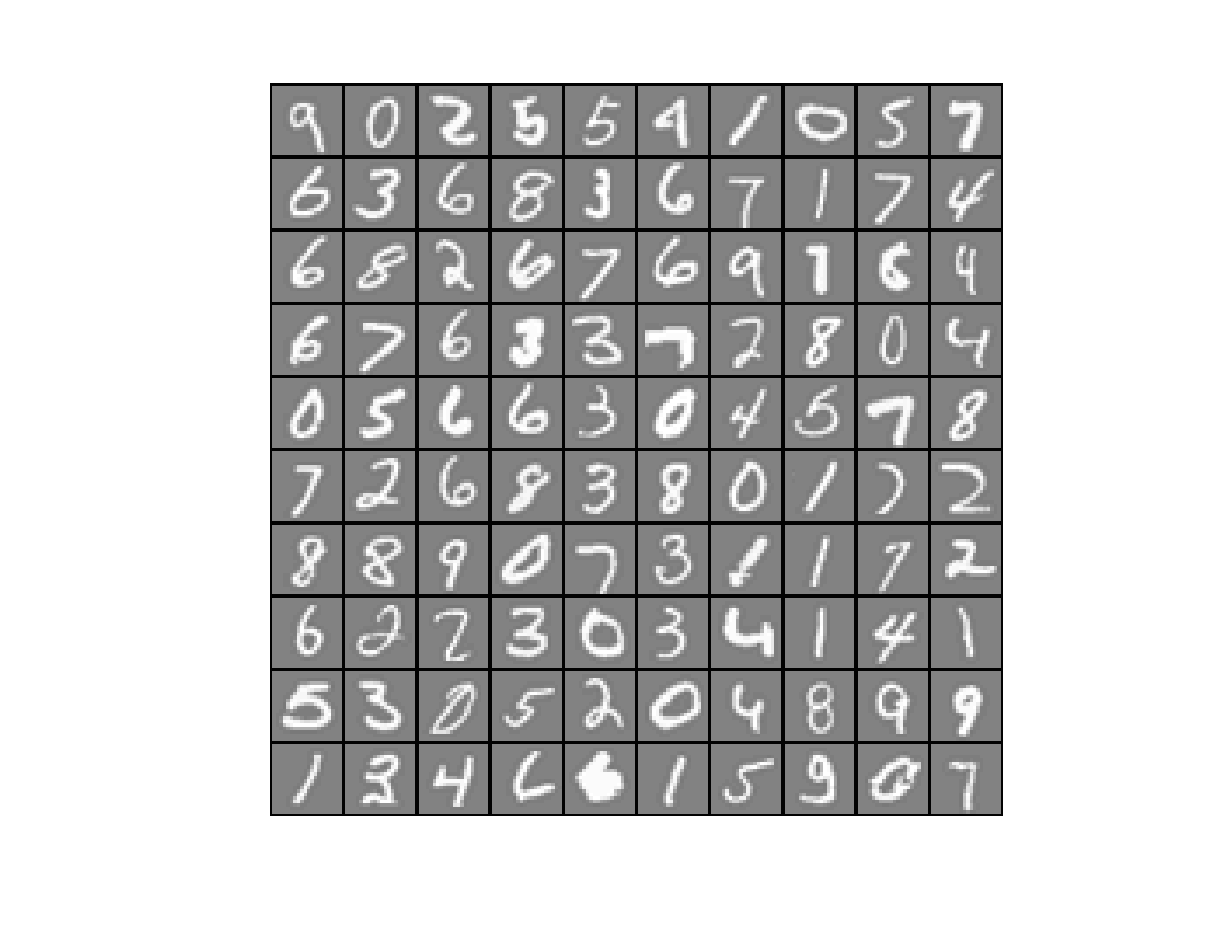
\includegraphics[width=.9\textwidth]{src/neuralNetwork2/nn}
\caption{Примероци од податочното множество}
\label{fig:neuralNetworkData}
\end{figure}

Податочното множество (дел е прикажан на слика \ref{fig:neuralNetworkData}) за овој алгоритам е
составено од 5000 тренинг примероци, од кој секој примерок е црно-бела слика од 20x20 пиксели. Секој пиксел се
репрезентира со децимален број кој го означува интензитетот. Овие 400 пиксели се
сместени во еднодимензионален вектор. Секој од овие тренинг примероци
претставува ред од матрицата X. Со ова се добива матрица од 5000 по 400 во која
секој ред е примерок за слика од ракописно напишана цифра.

\[
	X = \begin{bmatrix}
		    (x^{(1)})^T \\
			(x^{(2)})^T \\
			\vdots \\
			(x^{(m)})^T
			
		\end{bmatrix}
\]

Вториот дел од податочното множество е 5000-димензионален вектор $y$ кој 
ги содржи целните ознаки за податочното множество. За да се постигне
компатибилност со индексирањето во Octave/Matlab, каде што не постои 0 индекс,
цифрата 0 е пресликана во вредноста 10. Така, цифрата „0“ е означена како „10“,
додека цифрите од „1“ до „9“ се означени како „1“ до „9“ во нивниот природен
редослед.

\subsection{Репрезентација на моделот}

\begin{figure}[htb]
\centering
\includegraphics[width=.9\textwidth]{src/neuralNetwork2/neuralNetwork}
\caption{Моделот на невронска мрежа}
\label{fig:neuralNetwork}
\end{figure}

На слика \ref{fig:neuralNetwork} е прикажан моделот на невронската мрежа. Се
состои од 3 слоеви: влезен слој, скриен слој и излезен слој. На влезот на оваа
невронска мрежа се дигиталните слики. Затоа што секоја слика е со големина 20 x
20, влезниот слој е составен од 400 влезни единици.
